\scanpage{4}
\mspage{3}
Condition plus \unsure{fte|forte} : \deleted{\unsure{la topologie de $I$ est quotient pour}}
\inserted{(pour $\varphi$) l'application (continue \uline{surjection}) $\varphi$ est \uline{ouverte}}
\deleted{\unsure{celle de}}
\[
\begin{array}{rclcl}
\deleted{\unsure{X_\varphi\text{ est fidèle}|X_j\text{ est fermé}}}\ \Longleftrightarrow&
\varphi^{-1}(\overline J)&=&\overline{\varphi^{-1}(J)}&
\Longleftrightarrow\ \varphi^{-1}(\overline j)=\overline{\varphi^{-1}(j)}\quad\text{i.e.}\\
&\Vert&&\Vert&\\
&\displaystyle\bigcup_{j\in\overline J}X_j^*&&
\displaystyle\overline{\bigcup_{j\in J}X_j^*}=\bigcup_{j\in J}\overline{X_j^*}&
\end{array}
\]
\[
\overline{X_j^*}=\bigcup_{i\in\overline j}X_i^*\ (\overset{\mathrm{déf}}=X_j).
\]

Conditions pour une pseudo-partition $(X_i^*)_{i\in I}$ \inserted{loc. finie} indexée par un ens
pré\uline{ordonné} $I$, i.e. $\varphi:X\longrightarrow I$ application, en supposant $\varphi$ \uline{continue}
\deleted{que} les $X_i=\bigcup_{j\leq i}X_j^*$ fermés (donc les $X_i^*$ loc. fermés)

\unsure{2°|4°}) Top. de $I$ est finale pour $\varphi$ (i.e. quotient si $\varphi$ surjective) $\Longleftrightarrow$
\[
(X_J^*\text{ fermé}\Rightarrow J\text{ fermé})\Longleftrightarrow
(X_{\unsure{L|U}}^*\text{ ouvert})\Rightarrow\unsure{L|U}\text{ ouvert})
\]
\margin{si $\varphi$ surj. i.e. \unsure{1°|2°} $\Uparrow$}
3°) $\overline{X_j^*}=\bigcup_{\unsure{\underline{j}|\underset{\sim}{j}|j}\leq i}X_j^*$ pour tt $j\in I$ i.e. $\varphi$ est ouverte

1°) $\varphi$ surj i.e. les $X_i^*\ne\phi$
\margin{\uline{NB} Moyennant 1°, \unsure{7°|3°|2°}, on
récupère l'ordre de $I$ comme
la \unsure{relat|relation} d'inclusion entre les
$\overline{X_i^*}$ $\unsure{\mathinner{-\cdot\cdot}|\ldots}$}
\figure{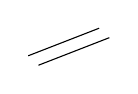
\begin{tikzpicture}[x=1cm,y=1cm]
\draw (0,0)--(0.9,0.35);
\draw (0.13,-0.12)--(1.03,0.23);
\end{tikzpicture}}

Une donnée $(X_i^*)_{i\in I}$ satisfaisant 1°) et 3°) équivaut à
$=$ : \unsure{d'une|une} relation d'équiv. \uline{loc\textsuperscript{t} finie} et \uline{ouverte}
\deleted{\unsure{telle que les classes soient|telle que les fermés soient}}
et $I$ est l'espace quotient (avec la relation de \inserted{pré}ordre
de spécialisation), \deleted{\illegible{3}} l'ens $I$ est \uline{ordonné} ssi
\[
(\forall i,j\quad\overline{X_i^*}=\overline{X_j^*}\Rightarrow i=j)
\Longleftrightarrow(\text{les }X_i\text{ sont loc. fermés}).
\]

\margin{cas $I$ \uline{ordonné} $\Updownarrow$}
\uline{Stratification} \uline{stricte}

famille loc finie \inserted{croissante} $(X_i)_{i\in I}$ de fermés, telle que $\forall j<i$
implique que $X_j$ rare dans $X_i$, et $\forall i,j\in I$,
on ait
\[
X_i\cap X_j=\bigcup_{k\in\overline i\cap\overline j}X_k.
\]
\figure{\begin{tikzpicture}\draw (0,0)--(2.4,0);\end{tikzpicture}}

Dans le cadre de la top. modérée, il faut voir comment
\inserted{pour} toute partition par des parties loc. fermées \uline{modérées},
il existe une plus petite \inserted{stratification modérée \unsure{strictes|\deleted{strictes}|\deleted{stricte}}}
\deleted{partition} \unsure{(formée)} \unsure{celles que|celles qui|telles que}
\deleted{\unsure{majorent|engendre}} la partition donnée.

% The following line records the ruled division between the two manuscript halves.
\figure{\begin{tikzpicture}\draw (0,0)--(0,-3);\end{tikzpicture}}
\mspage{4)}
\margin{\diagram{\begin{tikzcd}[x=0.65cm,y=0.65cm,
column sep=0pt,row sep=0pt,ampersand replacement=\&,
execute at end picture={
\node at (0,0) {$\overline{\unsure{J|I}}$};
\node at (1,0) {$\unsure{J|I}$};
\draw (1.65,-0.65)--(1.65,0.8);
\node at (2.6,0) {$y<x$};
\node at (2.18,1.45) {$\unsure{J|\supset}$};
\node at (2.18,0.8) {$\unsure{\Downarrow|\notin}$};
\node at (3.03,0.8) {$\in J$};
\draw (1.94,-0.4)--(2.09,-0.4);
\node at (5.2,0) {$x\in J$};
}]
{}
\end{tikzcd}}}

$(X_i^*)_{i\in I}$ une \inserted{partition indexée} \deleted{famille}
(loc. finie \inserted{de $X$} \deleted{\unsure{de parties disjointes de $X$, de réunion $X$, i.e. une $X\xrightarrow{\varphi}I$}}). Cond. équiv.

a) $\forall i\in I$, \deleted{\unsure{les $X_i^*\ne\phi$ (i.e. $\varphi$ surj, i.e. une partition), et}}
$\overline{X_i^*}$ est saturé \deleted{\unsure{pour les $X_i^*$ est loc. fermés|pour les $X_i^*$ et loc. fermés}}

b) $\exists\leq$ une \deleted{relation} \inserted{pré}ordre sur $I$, telle que l'on ait $\forall i\in I$
\[
\overline{X_i^*}=\bigcup_{j\in\overline i}X_j^*
\]
(\unsure{cette|\deleted{cette}} \deleted{relation} préordre est unique, \ldots
\[
i\leq j\Longleftrightarrow\overline{X_i^*}\subset\overline{X_j^*}\unsure{\rbrace|)}
\quad(\Longleftrightarrow X_i^*\subset\overline{X_j^*})
\]
c) La top. quotient de $I$ est telle que $\varphi:X\longrightarrow I$ soit ouverte,
i.e. $\forall U\in\operatorname{Ouv}(X)$, le saturé est ouvert

Sous ces conditions, la top. quotient de $I$ est celle
associée à \deleted{\unsure{sa relation d'ordre|la relation d'ordre}} préordre, qui est aussi
la relation de spécialisation pour cette topologie.
Pour que $I$ soit ordonné, il f. et s. que les
$X_i^*$ soient loc\textsuperscript{t}\unsure{.} fermés. On dit alors que la partition est
\uline{stratifiante} \unsure{(i.e. les $X_i^*$ saturés)|\deleted{(i.e. les $X_i^*$ saturés)}}.
\inserted{\unsure{les|\deleted{les}|\illegible{1}} loc. finie, pièces loc. fermées, relation d'équiv. ouverte}

On a une \uuline{correspondance} 1--1 entre les partitions
\inserted{stratifiantes} de $X$ de cette forme, i.e. les relations d'équiv. loc.
finies et ouvertes, \inserted{sur $X$, à fibres loc. fermées}, et l'ens des familles (à iso près)
$(X_i)_{i\in I}$ indexées par un ens. d'indices $I$ \uline{ordonné}
\inserted{\uline{loc. fini}},
qui sont telles que 1°) \unsure{famille|familles} \uline{\unsure{croissante|croissantes}} de parties
\inserted{\uline{fermées}} \deleted{\unsure{croissantes}} de $X$, \deleted{\unsure{et}} \uline{recouvrant} $X$, et 2°) $\forall i,j\in I$
\[
X_i\cap X_j=\bigcup_{k\in\overline i\cap\overline j}X_k
\]
\inserted{4°) \deleted{$\unsure{X_k|X_\alpha}$} $\forall i,j\in I$, $j<i$
$\Longrightarrow$ \deleted{\illegible{1}} $X_j$ \uline{rare} \uline{dans} $X_i$
\unsure{($\forall i$, i.e. $\unsure{X_i^*|\overline{X_i^*}}=X_i$)|(i.e. $\overline{X_i^*}=X_i$)}}
\inserted{3°) $\forall i$, $\underset{\substack{\Vert\,\mathrm{déf}\\X_i\setminus\bigcup_{j<i}X_j}}{X_i^*}\ne\phi$}

\margin{\uline{NB} Moyennant 1°, 2°, 4°, 3° équivaut à
la cond. plus faible
3 bis) $(\forall i\in I)$ $\unsure{X_i|X}\ne\phi$.}

Moyennant 1°) et 2°), en posant $X_i^*=X_i\setminus\bigcup_{j<i}X_j^*$,
les $X_i^*$ forment une \unsure{p.|ps.} partition \inserted{loc. finie} de $X$ par des
ens. loc. fermés; celle-ci satisfait les conditions
d'une \uline{partition} \uline{stratifiante} \uline{stricte}, \inserted{pour l'ordre donné à $I$} ssi
on a 3°) et 4°).

\uline{Stratification} : Conditions \unsure{1°) et 2°)|2°) et 1°)}. \uline{Strat. stricte} : ``fidèle'' (i.e.
3°) et condition de densité (4°) : Partitions \unsure{stratif.|stratifiantes} $\unsure{\Longleftarrow|\Longleftrightarrow}$ strat. \unsure{stricte|strictes}
\margin{3}
